%%%%%%%%%%%%%%%%%%%%%%%%%%%%%%%%%%%%%%%%%%%%%%%%%%%%%%%%%%%%%%%%%%%%%%%%%%%
%% This file is part of the book
%%
%% Algorithmic Graph Theory
%% http://code.google.com/p/graph-theory-algorithms-book/
%%
%% Copyright (C) 2009, 2010, 2011 Minh Van Nguyen <nguyenminh2@gmail.com>
%%
%% See the file COPYING for copying conditions.
%%%%%%%%%%%%%%%%%%%%%%%%%%%%%%%%%%%%%%%%%%%%%%%%%%%%%%%%%%%%%%%%%%%%%%%%%%%

\documentclass{article}

\usepackage{subfigure}
\usepackage{tikz}
\usetikzlibrary{external}
\tikzexternalize{grid-graphs}

\begin{document}

\begin{figure}
\subfigure[$2 \times 2$]{
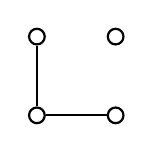
\begin{tikzpicture}
[lineDecorate/.style={-,thick},%
  nodeDecorate/.style={shape=circle,inner sep=2pt,draw,thick}]
%% nodes or vertices
\foreach \nodename/\x/\y in {0_0/0/0, 1_0/1/0, 0_1/0/1, 1_1/1/1}
{
  \node (\nodename) at (\x,\y) [nodeDecorate] {};
}
%% edges or lines
\path
\foreach \startnode/\endnode in {0_0/1_0, 0_0/0_1}
{
  (\startnode) edge[lineDecorate] node {} (\endnode)
};
\end{tikzpicture}
}
%%
%%
\qquad
\subfigure[$3 \times 3$]{
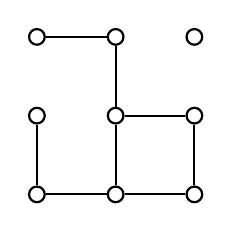
\begin{tikzpicture}
[lineDecorate/.style={-,thick},%
  nodeDecorate/.style={shape=circle,inner sep=2pt,draw,thick}]
%% nodes or vertices
\foreach \nodename/\x/\y in {
  0_0/0/0, 0_1/0/1, 0_2/0/2,
  1_0/1/0, 1_1/1/1, 1_2/1/2,
  2_0/2/0, 2_1/2/1, 2_2/2/2}
{
  \node (\nodename) at (\x,\y) [nodeDecorate] {};
}
%% edges or lines
\path
\foreach \startnode/\endnode in {
  0_0/1_0, 1_0/2_0, 0_0/0_1, 1_0/1_1, 2_0/2_1, 1_1/2_1, 1_1/1_2, 0_2/1_2}
{
  (\startnode) edge[lineDecorate] node {} (\endnode)
};
\end{tikzpicture}
}
%%
%%
\qquad
\subfigure[$4 \times 4$]{
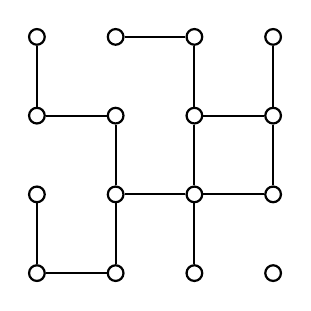
\begin{tikzpicture}
[lineDecorate/.style={-,thick},%
  nodeDecorate/.style={shape=circle,inner sep=2pt,draw,thick}]
%% nodes or vertices
\foreach \nodename/\x/\y in {
  0_0/0/0, 0_1/0/1, 0_2/0/2, 0_3/0/3,
  1_0/1/0, 1_1/1/1, 1_2/1/2, 1_3/1/3,
  2_0/2/0, 2_1/2/1, 2_2/2/2, 2_3/2/3,
  3_0/3/0, 3_1/3/1, 3_2/3/2, 3_3/3/3}
{
  \node (\nodename) at (\x,\y) [nodeDecorate] {};
}
%% edges or lines
\path
\foreach \startnode/\endnode in {
  0_0/0_1, 0_0/1_0, 1_0/1_1, 1_1/2_1, 2_0/2_1, 2_1/3_1, 1_1/1_2,
  2_1/2_2, 3_1/3_2, 0_2/1_2, 2_2/3_2, 0_2/0_3, 2_2/2_3, 3_2/3_3,
  1_3/2_3}
{
  (\startnode) edge[lineDecorate] node {} (\endnode)
};
\end{tikzpicture}
}
\end{figure}

\end{document}
